\section{Алгоритм программирования с экспрессией генов и его существующие модификации}

\subsection{Стандартный алгоритм}

\subsubsection{Алгоритм ПЭГ}

На рисунке~\ref{img:GEP_flowchart} показана блок-схема алгоритма ПЭГ~\cite{Ferreira2001}.

\begin{figure} [h]
\center
\begin{tikzpicture}[node distance = 5mm, every node/.style={transform shape}]
  \node [block] (create) {Создание начальной популяции};
  \node [block,    below = of create]   (express)  {Декодирование особей};
  \node [block,    below = of express]  (execute)  {Выполнение программ особей};
  \node [block,    below = of execute]  (evaluate) {Вычисление фитнеса особей};
  \node [decision, below = of evaluate] (condterm) {Останов};
  \node [block,    right = of condterm, xshift=1cm] (end) {Вернуть лучшую особь};
  \node [block,    below = of condterm, yshift=-1cm] (keepbest) {Копирование лучшей особи};
  \node [block,    below = of keepbest] (select)   {Отбор};
  \node [block,    below = of select]   (replica)  {Репликация};
  \node [block,    below = of replica]  (mutation)   {Мутация};
  \node [block,    below = of mutation] (transpos)   {Операторы переноса};
  \node [block,    below = of transpos] (recombin)   {Операторы рекомбинации};
  \path [line] (create) -- (express);
  \path [line] (express) -- (execute);
  \path [line] (execute) -- (evaluate);
  \path [line] (evaluate) -- (condterm);
  \path [line] (condterm) -- node [anchor=north] {Да}  (end);
  \path [line] (condterm) -- node [anchor=east] {Нет} (keepbest);
  \path [line] (keepbest) -- (select);
  \path [line] (select) -- (replica);
  \path [line] (replica) -- (mutation);
  \path [line] (mutation) -- (transpos);
  \path [line] (transpos) -- (recombin);
  \path [line] (recombin) -- ++(-4cm,0) |- (execute);
\end{tikzpicture}
\caption{Блок-схема исходного алгоритма ПЭГ}
\label{img:GEP_flowchart}
\end{figure}

Процесс начинается с конструирования популяции случайным образом созданных хромосом~\cite{ferreira:2001:wsc6Aa}. После экспрессии (декодирования) хромосом вычисляется фитнес каждой особи. На основании значений фитнеса особи отбираются и подвергаются изменениям, нацеленным на получение потомства~--- популяции с новыми характеристиками. С этой популяцией проводятся те же операции: декодирование генома, отбор, воспроизведение с модификациями. Процесс повторяется заданное количество итераций либо до обнаружения решения.

Воспроизведение включает в себя не только репликацию, но также выполнение генетических операторов, вносящих разнообразие. Во время репликации геном особи в точности, без изменений копируется и переносится в новое поколение. Очевидно, этот оператор не способен вносить разнообразие, потому требуется вмешательство оставшихся операторов, случайным образом выбирающих особи, к которым будут применены. Таким образом, в ПЭГ особь может быть модифицирована сразу несколькими операторами, а может оказаться и не изменённой вовсе.

%--------------------------------------------------------------------

\subsubsection{Открытые рамки считывания}

Структурная организация генома в ПЭГ более понятна в биологической терминологии открытых рамок считывания (open reading frames~--- ORF)~--- последовательностей генома, начинающихся стартовым кодоном, заверщающихся стоповым кодоном и содержащих кодирующие элементы между ними. В ПЭГ последовательность всегда начинается с первого элемента гена, но её конец не всегда совпадает с последним элементом. Таким образом, в ПЭГ нередка ситуация, когда участок от последнего элемента последовательности до конца гена не участвует в построении дерева, такие участки называют некодирующими.

В качестве примера рассмотрим следующее алгебраическое выражение:
\begin{equation}
\label{eq:GEP_sample_code_1}
\sqrt{(a+b)\times(c-d)}
\end{equation}

Выразить формулу~(\ref{eq:GEP_sample_code_1}) можно в виде синтаксического дерева, показанного на рисунке~\ref{img:GEP_ET_sample_1}:
\begin{figure} [h]
  \center
  \begin{tikzpicture}[level distance=1cm,
    level 1/.style={sibling distance=3cm},
    level 2/.style={sibling distance=2cm},
    level 3/.style={sibling distance=1cm}]
    \tikzstyle{every node}=[-,thick]
    \node { $\sqrt{}$ }
      child[->] { node { $\times$ }
        child { node { $+$ }
          child { node { $a$ } }
          child { node { $b$ } }
        }
        child { node { $-$ }
          child { node { $c$ } }
          child { node { $d$ } }
        }
      }
      ;
  \end{tikzpicture}
  \caption{Пример синтаксического дерева}
  \label{img:GEP_ET_sample_1}
\end{figure}

Количество ответвлений (дочерних узлов) у узлов, представляющих функцию, равно количеству аргументов этой функции. Узлы, соответствующие терминалам (переменным и константам) не имеют дочерних узлов. Изображённое дерево и является фенотипом особи в ПЭГ, в то время как генотип записывается следующим образом:

\begin{samepage}
\begin{verbatim}
01234567
Q*+-abcd,
\end{verbatim}
\end{samepage}

где очередность элементов обусловлена обходом графа в ширину. Это выражение является открытой рамкой считывания, в ПЭГ такие записи называются K-выражениями, а язык преобразования K-выражения в дерево и обратно~--- языком KARVA. Построение дерева из генома завершается, когда каждому ответвлению узла-функции поставлен в соответствие дочерний узел. Листья дерева, следовательно, являются терминалами.

Такая структура генома ПЭГ позволяет кодировать деревья различных размеров и форм, оперируя генами фиксированной длины, каждый из которых состоит из рамки считывания переменной длины и, при необходимости, некодирующего участка для заполнения пространства между концом кодирующей последовательности и концом гена. Хромосома особи состоит из одного или нескольких таких генов. Функция некодирующих участков, таким образом, состоит в обеспечении того, что длина рамки считывания всегда будет меньше или равна длине гена. Это позволяет гарантировать декодирование синтаксически правильного дерева после любых модификаций генома без ограничений и необходимости проведения сложных процедур проверки и редактирования. Отсутствие множества ограничений на генетические операторы является коренным отличием ПЭГ от~ГП.

%--------------------------------------------------------------------

\subsubsection{Геном в ПЭГ}

Каждый ген ПЭГ состоит из головы и хвоста. Голова содержит символы как функций, так и терминалов. Хвост содержит исключительно терминалы. Для каждой конкретной задачи подбирается длина головы гена $h$. Обозначим максимальное количество аргументов среди всех функций функционального множества как $n$, так для большинства арифметических функций $n=2$. Тогда маскимальную возможную длину хвоста гена $t$ можно вычислить по следующей формуле:

\begin{equation}
\label{eq:GEP_tail_size}
t(h,n) = h \times (n -1) + 1
\end{equation}

Ещё один параметр, требующий подбора под каждую задачу~--- количество генов (участков кода фиксированной длины, содержащих одно дерево) в хромосоме. Обычно используется больше одного гена, такие хромосомы называют мультигенными. Длина всех генов устанавливается равной для простоты применения операторов. Хромосома представляет собой символьную строку, полученную путём конкатенации всех генов.

Таким образом, ген~--- объект, состоящий из пяти атрибутов: $G = (E, T, F, Op, S)$, где $E$~--- генотип, $T$~--- терминальное множество, $F$~--- функциональное множество, $Op$~--- множество операторов, $S$~--- значение фитнеса на определённом элементе данных. Пример полной записи гена:

\begin{verbatim}
("*++-aabcd", "abcd", "+-*/", 0)
\end{verbatim}

Хромосома~--- объект, состоящий из четырёх атрибутов: $C = (G, T, L, Op, S)$, где $G$~--- набор генов, $L$~--- связующий оператор. Пример полной записи хромосомы:

\begin{verbatim}
C1=({G0, G1, G2}, "ab", +, "+-*/", 0.7)
\end{verbatim}

Пример символьной записи хромосомы:

\begin{samepage}
\begin{verbatim}
012345678 012345678 012345678
-b*babbab *Qb+abbba -*Qabbaba
\end{verbatim}
\end{samepage}

Данная хромосома содержит три гена, каждый из которых начинается с позиций, обозначенных индексом 0. Окончание рамки считывания каждого гена можно определить лишь после построения закодированного в нём синтаксического дерева; в приведённом примере декодирование первого гена завершается на позиции~4 (последний элемент), второго~---~5, третьего~---~5.

Каждое дерево может использоваться как по отдельности, с расчётом фитнеса для каждого гена, так и в совокупности, формируя более сложное дерево, фитнес которого и отражает приспособленность особи. Во втором случае каждое под-дерево является отдельной сущностью, компонентом иерархической структуры, представляющей б\'{о}льшую ценность, чем сумма её частей. Независимая друг от друга эволюция генов хромосомы как отдельных блоков иерархической системы при мультигенном подходе позволяет более эффективно решать сложные задачи.

Взаимодействие под-деревьев происходит с помощью связующих функций, для алгебраических выражений это, как правило, функция арифметического суммирования, для булевых~--- логическое ИЛИ. Обычно связующая функция устанавливается априори, однако может также быть добавлена в геном и выбираться в процессе эволюции. На рисунке~\ref{img:GEP_ET_sample_2} показано синтаксическое дерево, декодированное из рассматриваемой трёхгенной хромосомы с априорно заданной связью с помощью функции суммирования.

\begin{figure} [h]
  \center
  \begin{tikzpicture}[level distance=1cm,
    level 1/.style={sibling distance=3cm},
    level 2/.style={sibling distance=2cm},
    level 3/.style={sibling distance=1cm}]
    \tikzstyle{every node}=[-,thick]
    \node { $+$ }
      child[->] { node { $G_0$ }
        child { node { $-$ }
          child { node { $b$ } }
          child { node { $\times$ }
            child { node { $b$ } }
            child { node { $a$ } }
          }
        }
      }
      child[->] { node { $G_1$ }
        child { node { $\times$ }
          child { node { $\sqrt{}$ }
            child { node { $+$ }
              child { node { $a$ } }
              child { node { $b$ } }
            }
          }
          child { node { $b$ } }
        }
      }
      child[->] { node { $G_2$ }
        child { node { $-$ }
          child { node { $\times$ }
            child { node { $a$ } }
            child { node { $b$ } }
          }
          child { node { $\sqrt{}$ }
            child { node { $b$ } }
          }
        }
      }
      ;
  \end{tikzpicture}
  \caption{Пример дерева мультигенной хромосомы}
  \label{img:GEP_ET_sample_2}
\end{figure}

Такой простой способ кодирования синтаксических деревьев в виде линейных структур может быть использован и в других видах эволюционных алгоритмов, например, в иммунных сетях, как это показано в работе~\cite{karakasis2008efficient}.

%--------------------------------------------------------------------

\subsubsection{Функции фитнеса и отбор}

Одно из важнейших применений ПЭГ~--- символьная регрессия, цель которой~--- поиск выражения, наиболее соответствующего известным заданным значениям с определённой погрешностью. Установка небольшого значения (абсолютного или относительного) этой погрешности позволит обнаружить хорошие решения некоторых математических задач, однако в большинстве случаев маленькая допустимая погрешность замедляет эволюционирование по причине более строгого отбора особей. Если же задать слишком большую допустимую погрешность, отбор пройдёт множество особей, не являющихся приемлемыми решениями, однако значение фитнеса которых будет очень высоким.

Отбор особей в ПЭГ осуществляется пропорциональным оператором рулетки с простым элитизмом: лучшая особь популяции переносится в следующее поколение, шансы остальных прямо пропорциональны их фитнесу. Такая форма элитизма гарантирует, что лучшее обнаруженное решение не будет утрачено. Каждый запуск рулетки выбирает одну особь, соответственно, количество запусков рулетки равно размеру популяции.
После отбора новой популяции поочерёдно выполняются генетические операторы, применяемые к случайным образом выбранным особям. Например, если вероятность оператора составляет~70\%, то~7 из~10 особей будут им модифицированы. Каждая особь может быть модифицирована сразу несколькими операторами, однако оператор может быть применён к особи лишь однократно. Это отличает ПЭГ от~ГП, где особь не изменяется более чем одним оператором за итерацию. Получаемое таким образом потомство существенно отличается от родительских особей.

В ПЭГ применяются следующие операторы: репликации, мутации, копирования со сдвигом, копирования со двигом в корень, перестановки генов, одно- и двухточечной рекомбинации, генной рекомбинации. Рассмотрим каждый из них.

Репликация представляет собой самый простой оператор, не вносящий разнообразие в геном. Используется в паре с оператором отбора для копирования особей в новую популяцию в соответствии со значением фитнеса и случайностью, вводимой оператором рулетки.

Мутация (замена символа~--- элемента гена, соответствующего узлу дерева) может возникнуть в любом месте хромосомы. Вероятность оператора, как правило, задаётся эквивалентной двум мутациям в хромосоме. Элементы, подвергающиеся мутации в голове гена, могут быть изменены на любой другой символ (функцию или терминал), в хвосте~--- только на терминал. Данное ограничение нацелено на сохранение структуры хромосомы и обеспечение декодирования синтаксически верного дерева. Среди всех модифицирующих операторов мутация является самым важным и эффективным, т.к. в отличие от остальных, комбинирующих существующие участки генома, мутация направлена на создание новых элементов, а потому вносит наиболее радикальные изменения, расширяя область поиска решений.

Следующие три оператора перемещают последовательные участки генома в пределах хромосомы. Три типа таких участков накладывают различные ограничения на операторы.

Оператор копирования со сдвигом копирует последовательность символов генома в любую позицию головы гена, кроме первой. Ограничение на первую позицию обусловлено тем, что перемещаемая последовательность может начинаться с терминального символа, помещение которого в корень приведёт к вырожденному дереву из одного элемента. Ген-источник копируемой последовательности остаётся неизменным. Элементы головы гена-приёмника начиная с позиции, в которую будет скопирована целевая последовательность, сдвигаются для освобождения места, вышедшие за пределы головы элементы отбрасываются.

Оператор копирования со сдвигом в корень отличается от предыдущего тем, что целевая последовательность начинается с элемента-функционала и копируется в корень гена-приёмника. Оба оператора копирования вносят значительные изменения, и потому наравне с мутацией отлично подходят для внесения генетического разнообразия, предотвращая застревание в локальном оптимуме и ускоряя поиск хороших решений.

Оператор перестановки генов вносит изменения в результат вычисления декодированного дерева только при условии использования некоммутативной связующей функции в мультигенной хромосоме, такой как <<ЕСЛИ, ТО>>. Однако более всего преобразующая сила данного оператора проявляет себя в связке операторами кроссовера. Например, возможно появление дублирующихся генов~--- явление, играющее важную роль в биологии и эволюции.

Все три вида рекомбинации производят обмен генетическим материалом между двумя родительскими хромосомами, порождая две новые особи. Вероятность того, что будет применён один из трёх описанных ниже операторов обычно задают~70\%.

В операторе одноточечной рекомбинации две особи скрещиваются вокруг линии, проходящей через случайным образом выбранную позицию хромосомы. Рассмотрим на примере двух родительских хромосом:

\begin{samepage}
\begin{alltt}
012345012345
XXXXXXXXXXXX
OOOOOOOOOOOO
\end{alltt}
\end{samepage}

Взяв для примера позицию~3 в первом гене как точку кроссовера, оператор меняет местами участки хромосом особей от точки кроссовера между собой, что выглядит следующим образом:

\begin{samepage}
\begin{alltt}
012345012345
XXXOOOOOOOOO
OOOXXXXXXXXX
\end{alltt}
\end{samepage}

В большинстве случаев полученное потомство проявляет характеристики своих родителей, что делает одноточечную рекомбинацию наиболее часто используемым в ПЭГ оператором, наравне с мутацией.

Отличие двухточечной рекомбинации состоит в том, что обмен участками генома происходит между двумя точками. Выбрав в качестве примера позицию~2 в первом гене и~4~--- во втором, и применив оператор, дочерние хромосомы выглядят как описано ниже:

\begin{alltt}
012345012345
XXOOOOOOOOXX
OOXXXXXXXXOO
\end{alltt}

Преобразующая сила (способность вносить генетическое разнообразие) двухточечной рекомбинации выше, чем у одноточечной, потому применяется чаще для решения сложных задач с использованием мультигенных хромосом.

В генной рекомбинации производится замена генов, занимающих в обоих хромосомах позицию, определяемую случайным образом.

Следует отметить, что использование рекомбинации и/или операторов перемещения как единственного вида применяемых операторов сводится к перемешиванию существующих участков генома, и не обеспечивает создание нового генетического материала. Потому для решения сложных задач в таком случае может понадобиться популяция большого размера. Созидательная способность ПЭГ заключается в применении всех описанных техник.

%--------------------------------------------------------------------

\subsubsection{Методика тестирования}

Для проведения экспериментов была реализована система ПЭГ на языке программирования C, принимающая в качестве аргумента файл с набором точек (заданных координатами) и выдающая лучшую обнаруженную формулу, набор точек~--- модель, полученную с использованием этой формулы, и динамику среднеквадратичной ошибки лучшей особи с течением времени. В исходный алгоритм затем поочерёдно добавлялись описанные далее модификации, с возможностью включения и выключения каждой из них в любых комбинациях.  Так, например, при каждом запуске можно выбрать оператор селекции (рулетка, отбор по плотности либо турнир), вероятность мутации, способ кодирования и т.п.

Рандомизированная природа алгоритма ПЭГ приводит к необходимости использовать статистические методы для оценки его эффективности. Для этого каждая исследуемая комбинация модификаций алгоритма запускалась множество раз (обычно 100), анализу подвергались значения СКО лучших моделей, полученных в ходе каждого запуска. Наиболее интересными показателями являются: СКО наилучшей модели среди всех запусков ($e_{b}$), средний СКО ($e_{m}$), доля успешных запусков ($r_{f}$)~--- таких, в ходе которых была получена модель с приемлемой для данной задачи точностью.

Было обнаружено, что в большинстве случаев подбор комбинаций параметров и модификаций позволяет добиться улучшения какой-либо одной из характеристик $e_{b}$ и $r_{f}$, но не обеих одновременно. Направленность на снижение $e_{b}$ наиболее оправдано в тех случаях, когда процесс поиска модели не стеснён во времени, а целью является получение как можно более точной модели. Повышение доли успешных запусков $r_{f}$ является целью при поиске оптимального алгоритма решения задач, требующих быстрого построения моделей с приемлемой заданной точностью.

Таким образом, $e_{b}$ отражает способность алгоритма к обнаружению лучшей из возможных моделей, а $r_{f}$~--- вероятность получения модели достаточной точности при очередном запуске алгоритма.

Сравнение систем, собранных с различными параметрами, проводилось на трёх задачах поиска формул, описывающих такие модели:
\begin{enumerate}
  \item $y(x) = \sin x, x \in [-5, 4.6]$;
  \item Функция Розенброка: $z(x, y) = {(1 - x)}^2 + 100 {(y - x^2)}^2, x \in [-3, 3], y \in [-3, 3]$;
  \item Сумма четырёх сигмоид:
    \begin{multline}
      z(x, y) = \frac{1}{2} \times e^{-\left\lbrack\cfrac{(9x-2)^2 + (9y-2)^2}{4}\right\rbrack} + \frac{3}{4} \times e^{-\left\lbrack\frac{(9x+1)^2}{49} + \frac{(9y+1)^2}{10}\right\rbrack} + \\
      + \frac{1}{2} \times e^{-\left\lbrack\frac{(9x-7)^2 - (9y-3)^2}{4}\right\rbrack} -\frac{1}{5} \times e^{-\left\lbrack(9x-4)^2 + (9y-7)^2\right\rbrack}, \\
      x \in [-2, 2], y \in [-2, 2]
    \end{multline}
\end{enumerate}

При моделировании функций синуса и Розенброка использовалось функциональное множество, состоящее из четырёх арифметических действий, в последнем случае~--- полное множество, в состав которого входят арифметические (сложение, вычитание, умножение, деление), тригонометрические ($\sin$, $\cos$, $\tan$, $\sinh$, $\cosh$, $\tanh$), степенн\'{ы}е (возведение в степень, взятие квадратного корня, экспонента, логарифм). Полученные с применением этих формул модели изображены на рисунке~\ref{img:functionz}. Значения приемлемых СКО моделей, при которых задача будет считаться решённой, составляют для этих задач, соответственно, 0.08, 0.05 и 0.06.

\begin{figure} [h]
  \center
  \begin{subfigure}[t]{0.3\linewidth}
    \center
    \begin{tikzpicture}[domain=-5:4.6]
      \begin{axis}[width=\linewidth, title={$y=\sin{x}$}, no marks]
        \addplot{sin(deg(x))};
      \end{axis}
    \end{tikzpicture}
  \end{subfigure}
  \begin{subfigure}[t]{0.3\linewidth}
    \center
    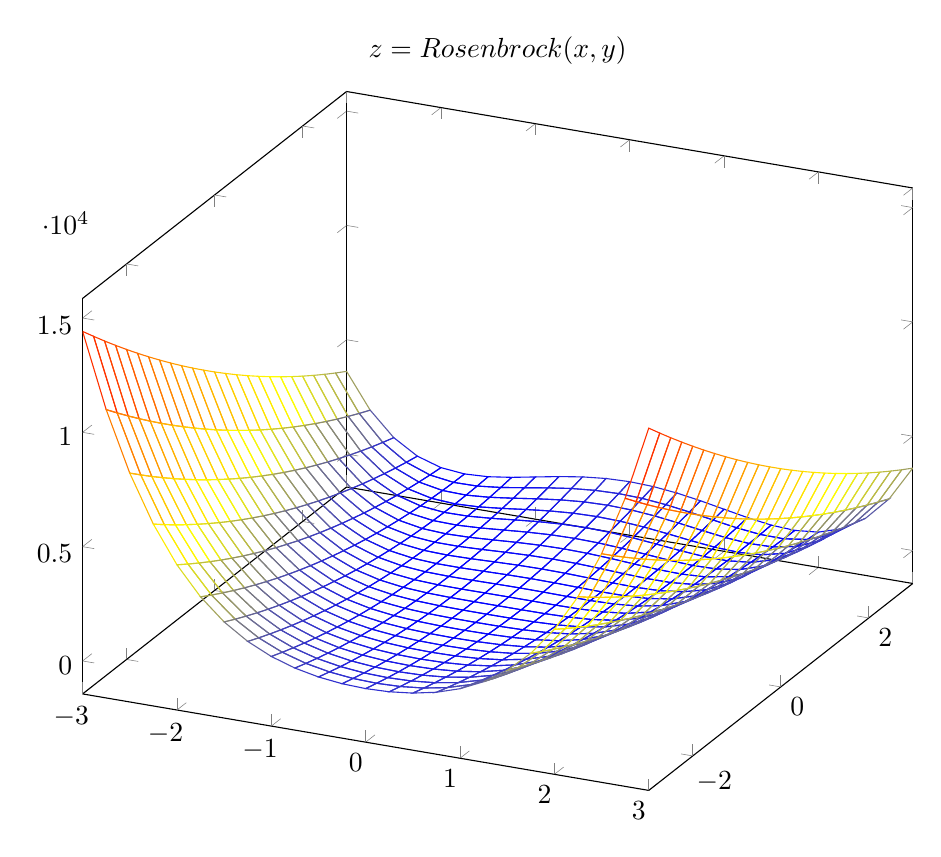
\begin{tikzpicture}
      \begin{axis}[width=\linewidth, title={$z=Rosenbrock(x, y)$}]
        \addplot3[mesh, domain=-3:3]{(1 - x)^2 + 100 * (y - x^2)^2};
      \end{axis}
    \end{tikzpicture}
  \end{subfigure}
  \begin{subfigure}[t]{0.3\linewidth}
    \center
    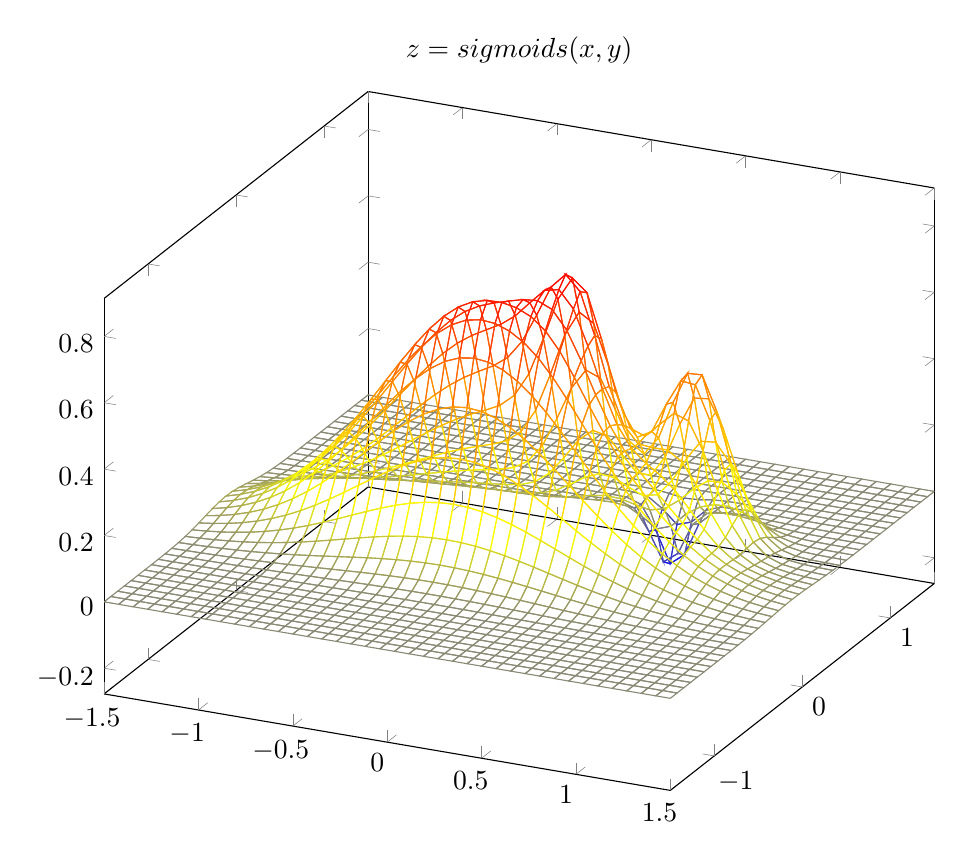
\begin{tikzpicture}
      \begin{axis}[width=\linewidth, title={$z=sigmoids(x, y)$}]
        \addplot3[mesh, samples=40, domain=-1.5:1.5]{0.5 * e^(- (((9*x-2)^2) + ((9*y-2)^2)) / 4) + 0.75 * e^(- ((9*x+1)^2) / 49 - ((9*y+1)^2) / 10) + 0.5 * e^(- (((9*x-7)^2) + (9*y-3)^2) / 4) -0.2 * e^(-  ((9*x-4)^2) - (9*y-7)^2)};
      \end{axis}
    \end{tikzpicture}
  \end{subfigure}
  \caption{Тестовые модели}
  \label{img:functionz}
\end{figure}

%--------------------------------------------------------------------

\subsubsection{Влияние оператора мутации на динамику эволюции}

Процесс эволюции основан на генетической изменчивости и процедуре отбора. Эти же механизмы задействованы во всех эволюционных алгоритмах. Однако способ обеспечения генетической изменчивости, который можно было бы назвать лучшим, не был выявлен. Исследователи разделяют эти способы на мутацию и рекомбинацию. Успешность эволюции также сильно зависит от применяемых алгоритмом генетических операторов, размера и состава начальной популяции.

Сравнивая эффективность исходного алгоритма ПЭГ при разных размерах популяции следует учесть, что время выполнения алгоритма прямо пропорционально размеру популяции. Рассмотрим для начала случай, когда работа алгоритма не ограничена во времени выполнения, результаты такого эксперимента приведены в таблице~\ref{tbl:cmp_pop_sizes_no_time_limit}. Можно заметить, что размер популяции больше 100 не даёт прироста характеристик.

\input{cmp_pop_sizes_no_time_limit}

Для оценки данного фактора в условиях ограниченного времени время каждому запуску было отведено фиксированное время работы, потому алгоритмы с б\'{о}льшим размером популяции имели возможность расчитать меньшее число поколений. Результаты продемонстрированы в таблице~\ref{tbl:cmp_pop_sizes}, из которых также следует наличие пика эффективности при размере популяции 40~особей.

\input{cmp_pop_sizes}

В системах на основе генотипа и фенотипа пространство поиска отделено от пространства решений, что существенно улучшает производительность таких систем. Чем меньше ограничений накладывается на процедуру проецирования генотипа на фенотип и обратно~--- тем более эффективна система, т.к. практически любой оператор может быть использован для исследования пространства поиска, включая мутацию.

Так, например, в системе DGP (Developmental Genetic Programming~--- ГП с развитием~\cite{poli2008field}) в результате трансляции генотипа в фенотип не всегда получается синтаксически верное дерево, что приводит к необходимости проведения дополнительных операций по устранению непригодных особей. Потому мутация в DGP не превосходит по показателям операторы кроссовера.

Для сравнения эффективности каждого из генетических операторов, применяемых в ПЭГ, по отдельности были сопоставлены динамические данные процесса эволюции: графики фитнеса лучшей особи с течением поколений (итераций), и графики среднего фитнеса популяции~\cite{ferreira:2002:FEA}.

В ходе поиска модели, созданной формулой $y(x) = x^4 + x^3 + x^2 + x$ была исследована динамика эволюционного процесса с различными значениями вероятности применения оператора мутации ($p_{m_1}, p_{m_2}, p_{m_3}, p_{m_4}$), значения фитнеса приведены на рисунке~\ref{img:cmp_health}.

\begin{figure} [h]
  \center
  \begin{subfigure}[h]{0.3\linewidth}
    \center
    \begin{tikzpicture}
      \begin{axis}[title={а) $p_{m_1} = 0$}, width=\linewidth, no marks, ymax = 1000, ylabel={Фитнес}, xlabel={Время, мс}, legend entries={{Лучший фитнес},{Средний фитнес}}, legend to name=legend_local_refcmp_health, legend columns=2]
        \addplot[mark=x,red] table[x=time,y=best] {data_to_plot/health_0};
        \addplot[mark=*,blue] table[x=time,y=mean] {data_to_plot/health_0};
      \end{axis}
    \end{tikzpicture}
  \end{subfigure}
  \begin{subfigure}[h]{0.3\linewidth}
    \center
    \begin{tikzpicture}
      \begin{axis}[title={б) $p_{m_2} > p_{m_1}$}, width=\linewidth, no marks, ymax = 1000, ylabel={Фитнес}, xlabel={Время, мс}]
        \addplot[mark=x,red] table[x=time,y=best] {data_to_plot/health_1};
        \addplot[mark=*,blue] table[x=time,y=mean] {data_to_plot/health_1};
      \end{axis}
    \end{tikzpicture}
  \end{subfigure}
  \\
  \begin{subfigure}[h]{0.3\linewidth}
    \center
    \begin{tikzpicture}
      \begin{axis}[title={в) $p_{m_3} > p_{m_2}$}, width=\linewidth, no marks, ymax = 1000, ylabel={Фитнес}, xlabel={Время, мс}]
        \addplot[mark=x,red] table[x=time,y=best] {data_to_plot/health_2};
        \addplot[mark=*,blue] table[x=time,y=mean] {data_to_plot/health_2};
      \end{axis}
    \end{tikzpicture}
  \end{subfigure}
  \begin{subfigure}[h]{0.3\linewidth}
    \center
    \begin{tikzpicture}
      \begin{axis}[title={г) $p_{m_4} > p_{m_3}$}, width=\linewidth, no marks, ymax = 1000, ylabel={Фитнес}, xlabel={Время, мс}]
        \addplot[mark=x,red] table[x=time,y=best] {data_to_plot/health_3};
        \addplot[mark=*,blue] table[x=time,y=mean] {data_to_plot/health_3};
      \end{axis}
    \end{tikzpicture}
  \end{subfigure}
  \\
  \ref{legend_local_refcmp_health}
  \caption{Динамика эволюции при разных вероятностях мутации}
  \label{img:cmp_health}
\end{figure}



На рисунке~\ref{img:cmp_health}а видно, что график лучшего фитнеса практически совпадает с графиком среднего фитнеса, особенно в поздних поколениях. Такие популяции называются умеренно инновационными в силу небольшого разнообразия между особями и медленного процесса эволюции. Вероятность успешного обнаружения решения задачи, поставленной в эксперименте, составила~16\% (отношение запусков, в ходе которых решение было обнаружено, к общему количеству запусков алгоритма).

На следующем рисунке заметно, что форма графиков совпадает (не принимая во внимание колебания графика среднего фитнеса), однако они не пересекаются, между ними наблюдается разрыв. Процентное соотношение успешных запусков составило~47\%. Такая модель эволюции является здоровой, но слабой.

С повышением вероятности мутации возрастает успешность алгоритма, достигая максимума при $p_{m_3}=0.1$, показанного на рисунке~\ref{img:cmp_health}в: здоровая и сильная модель. Характерен б\'{о}льший разрыв между графиками, чем в предыдущем случае, однако с сохранением тенденции к росту среднего фитнеса.

Наконец, последняя приведённая динамика со средним фитнесом на постоянном низком уровне с небольшими колебаниями является примером полностью хаотической системы, в которой, несмотря на элитизм, каждое поколение является по сути случайным.

Исследование операторов рекомбинации в качестве единственных источников, вносящих генетическое разнообразие, выявило процесс усреднения популяции~--- быстрое сокращение разрыва между графиками лучшего и среднего фитнеса с последующим их перекрытием. Это означает, что геном всех особей популяции совпадает, и разнообразие устранено, что является следствием преждевременной сходимости такого подхода к локальному оптимуму.

В начальной популяции, заполненной особями, созданными случайным образом, жизнеспособные решения~--- событие редкое, особенно при решении сложных задач. Удачным подходом в таком случае будет начало процесса эволюции с одной или нескольких особей-основателей~\cite{HreFer02}. Эффект основателя, описанный Э.~Майром, как создание новой популяции из особей-основателей, может быть инициирован дрейфом генов~--- изменением частоты вариантов генов вследствие случайных процессов и работы операторов отбора. Наиболее выраженный случай эффекта основателя~--- колонизация необитаемой области (создание новой популяции) одной особью.

Это означает, что при определённом значении вероятности мутации можно добиться максимальной эффективности работы всего алгоритма. Кроме того, оператор мутации уменьшает тенденцию популяции к гомогенизации (утрате разнообразия), и устраняет сильную зависимость эффективности алгоритма от размера популяции.

Влияние вероятности мутации на эффективность алгоритма показано в таблице~\ref{tbl:cmp_mutation_probabilites}. При рассмотрении результатов эксперимента можно заменить выраженный пик эффективности в 1-2~мутации на хромосому (в зависимости от задачи).

\input{cmp_mutation_probabilites}

%--------------------------------------------------------------------

\subsubsection{Нейтральные гены}

После декодирования хромосомы ПЭГ и конструирования синтаксического дерева количество узлов полученного дерева в предельном случае будет равно размеру хромосомы, однако в большинстве случаев будет меньшим. Те элементы в хвостах генов, которые не были использованы при построении дерева, называются некодирующими участками. Кроме того, полученное дерево может содержать выражения вида $(a - a)$, $(a \times 0)$, $(a - 0)$ и т.п., которые при семантическом анализе упрощаются, устраняя данные интроны и образуя более компактное дерево. Множество подобных участков~--- часто повторяющихся последовательностей, интронов, псевдогенов и пр.~--- встречается в природе в ДНК живых существ. Потому логично предположить, что и в искусственном геноме нейтральные участки могут быть полезны. Среднее количество нейтральных последовательностей в популяции растёт с увеличением как количества генов в хромосоме, так и размера каждого из них.

Исследования работы алгоритма с различной длиной генома показали~\cite{journals/advcs/Ferreira02}, что эволюционирование особей с высокой степенью избыточности генома происходит эффективней. Это связано с тем, у каждого решения, представленного в наиболее компактной форме, существует множество менее компактных вариантов представления, увеличенных в размерах за счёт интронов. Кроме того, накапливаемые в некодирующих участках мутации могут быть задействованы в дальнейшем, если изменения в голове гена (добавление функциональных узлов) приведут к увеличению размера дерева. В таблице~\ref{tbl:cmp_chrom_sizes} приведены результаты моделированя с различной длиной генома. Удлиннение генома ведёт к возрастанию пространства поиска, появлению деревьев б\'{о}льшего размера, следовательно, ведёт к более длительному расчёту популяции. Имеет смысл сравнивать модели, на построение которых было затрачено равное время. В приведённой таблице видно, что для каждой задачи имеется некая оптимальная длина генома. Меньший размер генов не позволяет выразить деревья достаточной сложности, а при б\'{о}льшем требуется на порядки больше вычислительного времени.

\input{cmp_chrom_sizes}

%--------------------------------------------------------------------

\subsubsection{Сведение к ГА}

Простейшим представлением генома в ПЭГ является ген, состоящий из одного терминала. Организация хромосомы, состоящей из одноэлементных генов делает ПЭГ эквивалентным ГА. Однако для решения комбинаторных задач требуются особые связывающие функции, отличные от простых арифметических и булевых. Например, для задачи коммивояжёра связь отображает расстояние между городами, представленными соответствующими генами. Если обозначить каждый город из девяти отдельным символом, то следующая хромосома из девяти элементов представит один из возможных путей обхода:

\begin{verbatim}
CADEBHFIG
\end{verbatim}

Если оптимизационная задача содержит $N$ классов терминалов, хромосома может состоять из $N$ групп одноэлементых генов, называемых мультигенными группами (МГГ~--- multigene family, MGF)~\cite{ferreira:2002:ASIA}. Например, при отображении одного шестиэлементного множества $\{1, 2, 3, 4, 5, 6\}$ в другое $\{A, B, C, D, E, F\}$ хромосома будет состоять из двух шестиэлементных групп:

\begin{samepage}
\begin{verbatim}
012345 012345
632451 EDFCBA
\end{verbatim}
\end{samepage}

Особенностью МГГ является то, что она не содержит повторяющихся элементов, а отображает перестановку элементов некоторого конечного множества. Потому операторы мутации и рекомбинации к такой структуре генома неприменимы из-за возможности некорректных последовательностей с повторяющимися и отсутствующими элементами. Следовательно, для внесения генетического разнообразия должны быть созданы новые операторы, порождающие корректные структуры.

Один из таких операторов~--- инверсия, впервые описанная Холландом в 1975 году. Случайным образом выбирается участок МГГ и изменяется порядок следования элементов в нём. Так, например, результатом применения к хромосоме из предыдущего примера может стать следующий геном:

\begin{samepage}
\begin{alltt}
012345 012345
632451 E{\underline{CFD}}BA
\end{alltt}
\end{samepage}

Из проведённых экспериментов следует, что оператор инверсии обладает более сильной изменяющей способностью и, следовательно, наиболее способствует скорейшему обнаружению решения.
Оператор перемещения гена располагает случайным образом выбранный ген по другой позиции, сохраняя порядок следования остальных генов группы. Использование данного оператора вместе с более мощными, такими как инверсия, может быть полезно для точной подстройки решения. Однако эксперименты показали, что эффективность инверсии, используемой в одиночку, более эффективно.

Оператор перестановки генов меняет местами два случайным образом выбранных гена в пределах МГГ. Исследование оператора перемещения участков гена показало его крайнюю неэффективность~--- особи-потомки имели, как правило, худший фитнес, чем родительские особи.

%--------------------------------------------------------------------

\subsection{Числовые константы в ПЭГ}

Создание числовых констант с плавающей запятой необходимо для выполнения символической регрессии. В исходном алгоритме ПЭГ для обозначения константы в геноме используется терминальный символ <<?>>, а начальный набор констант представлен доменом $D_c$~\cite{ferreira:2002:WSC}. Каждый ген располагает собственным массивом, содержащим используемые им константы, этот массив заполняется на основе домена $D_c$ при генерации начальной популяции. Численное значение константным символам назначается только при экспрессии генов. Для внесения генетического разнообразия был добавлен специальный оператор мутации констант.

Начальный набор возможных численных констант может быть задан вручную: как перечислением, так и заданием диапазона~--- успешное решение задач таким методом прямого управления константами возможено только при наличии априорных знаний о решении, позволяющих задать корректный диапазон. Потому на практике используется другой метод, который заключается в инициализации значений констант случайными числами.

%--------------------------------------------------------------------

\subsubsection{Динамическая мутация}

При старте алгоритма ПЭГ на этапе создания новой популяции начальные значения констант в хромосомах предлагается отбирать из множества $A$=\{0.1316, 0.2128, 0.3441, 0.5571, 0.9015, 1.4588, 2.3605, 3.8195, 6.1804, 10.0007\}, созданного таким образом, чтобы соотношение соседних элементов являлось золотым сечением~\cite{Peng:2007:FFC:1304604.1305824}. В данной модификации предлагается следующий оператор мутации констант. Для каждой константы~$C_j$ в геноме выбранной особи:
\begin{enumerate}
  \item Из фиксированного глобального массива первичных констант~A случайным образом выбирается константа~$V$.
  \item Случайным образом выбирается оператор~$Op$ из множества~$\{+, -, /, *$\}.
  \item $C_j \leftarrow Op(C_j, V)$.
\end{enumerate}

%--------------------------------------------------------------------

\subsubsection{Плавная и случайная мутация}

В работе~\cite{li:2004:lbp} описаны исследования операторов мутации, основанных на техниках плавной и случайной мутации. Был задан оператор одноточечной мутации константы: при начальной конфигурации ПЭГ задаётся отсортированный список возможных констант. Данный оператор изменяет одну символ-константу в гене, при случайной мутации на замену выбирается любой другой элемент списка, при плавной~--- какой-либо из соседних текущему. Данная операция применяется к каждому гену хромосомы. Локальный поиск должен производиться в сторону оптимального решения, это означает применение результата мутации только тогда, когда её результат повышает фитнес особи.

Всего было исследовано пять подходов к мутации:
\begin{enumerate}
  \item Плавная мутация лучшей особи в конце расчёта поколения.
  \item Случайная мутация лучшей особи в конце расчёта поколения.
  \item Плавная мутация каждой особи в первые $\alpha\%$~поколений в конце расчёта поколения.
  \item Случайная мутация каждой особи в первые $\alpha\%$~поколений в конце расчёта поколения.
  \item Интервальная случайная мутация: первые $g$~поколений случайной мутации подвергаются все особи популяции в конце расчёта поколения.
\end{enumerate}

Применение подхода, при котором мутации подвергается только лучшая особь поколения, никак не повлияло на эффективность алгоритма. Из этого можно сделать вывод, что лучшая особь, полученная исходным алгоритмом ПЭГ, является по определению достаточно хорошей и не требует модификаций. Также это подтверждает, что решающую роль в поиске оптимальных решений играет именно эволюционный процесс ПЭГ: выполнение генетических модификаций и отбор.

Применение мутации к каждой особи популяции значительно повышает фитнес популяции, особенно в первых поколениях. Однако с течением времени процентное соотношение особей, улучшенных после мутации, падает. Это происходит вследствие того, что спустя определённое количество поколений формируются группы суб-оптимальных решений, константы которых уже должным образом настроены, потому на этом этапе важнее операторы, приводящие к б\'{о}льшим изменениям.

Задействование методов, применяющих мутации констант к каждой особи, влечёт за собой повышение времени выполнения алоритма, однако получение более качественных решений не позволяет напрямую сравнить эффективность таких модифицированных алгоритмов с исходным ПЭГ. Кроме того, применение указанных трёх техник к различным задачам не позволило выявить наилучшую из них.

На практике была применена авторская модификация~--- плавно-динамическая мутация,~--- описанная далее. Сравнение эффективности описанных мутаций констант приведено в таблице~\ref{tbl:cmp_dynamic_mutation}.

\input{cmp_dynamic_mutation}

%--------------------------------------------------------------------

\subsection{Модификации процедур кодирования дерева}

\subsubsection{Префиксное кодирование}

В исходном алгоритме ПЭГ декодирование дерева производится путём линейного извлечения элементов генома и установки в узлы формируемого дерева при его обходе в ширину. При замене обхода дерева в ширину обходом в глубину повышается связность генома~--- уменьшается расстояние между элементами, соответствующими соседним узлам дерева, а под-дерево кодируется непрерывной строкой в геноме. Такой подход способствует сохранению субструктур, что делает менее разрушительным применение операторов скрещивания~\cite{Li:gecco05lbp}. Сохранение в популяции субструктур (суб-деревьев) лучших особей и их рекомбинация позволяет ускорить сходимость алгоритма: оптимальное решение обнаруживается на более ранних поколениях (в несколько раз быстрее), качество оптимального решения зачастую выше, чем результат работы оригинального алгоритма ПЭГ.

Однако при таком подходе разрушается гарантия получения синтаксически корректного дерева из любого генома, сформированного согласно правилам. Потому требуется ввести процедуру динамической валидации дерева. К участию в эволюционном процессе допускаются только те особи, декодирование которых порождает корректное дерево. Такая система получила название P-GEP.

От предыдущих авторов. Предложенная линейная структура генома делает возможнным легко выделять из него отдельные под-деревья, что, в свою очередь, позволяет производить поиск повторяющихся субструктур. Появление часто встречающихся субструктур в лучших особях популяции означает их высокую полезность при составлении конечного решения. Выделив набор таких субструктур популяции авторами предлагается формировать из них т.н. элитную группу~\cite{Substructures(ICMLA05)_XLi}. Каждый элемент этой группы обозначается одним дополнительным терминальным символов.

Для взаимодействия между особями и элитной группой были введены два новых генетических оператора: оператор сжатия, заменяющий последовательность в геноме особи соответствующим терминальным символом из элитной группы, и оператор раскрытия, выполняющий обратную операцию~--- замену терминального символа на соответствующую последовательность из элитной группы.
Внесение данной модификации в P-GEP привело к обнаружению решений, имеющих значительно меньшую погрешность.

Для последующего применения важно определить влияние таких базовых параметров, как вероятность мутации, на данную модификацию алгоритма, результаты эксперимента приведены в таблице~\ref{tbl:cmp_mutations_prefix}. Отметим максимум эффективности при~1-2~мутациях на хромосому, аналогично при кодировании путём обхода графа в ширину.

\input{cmp_mutations_prefix}

%--------------------------------------------------------------------

\subsubsection{Кодирование с наложениями}

В работе~\cite{conf/icnc/PengTZY05} рассматривается разновидность декодирования генома путём обхода дерева в глубину, при котором последовательно идущие под-деревья накладываются друг на друга. Элементы генома последовательно считываются:
\begin{itemize}
  \item Если текущий символ принадлежит к терминальному множеству~--- поместить его в синтаксическое дерево как листовой узел.
  \item Если текущий символ принадлежит к функциональному множеству~--- поместить его в синтаксическое дерево как узел с количеством дочерних узлов, равным количеству аргументов помещаемой функции. Первый дочерний узел~--- следующий в геноме за текущим, второй~--- следующий за ним и т.д. Дочерние под-деревья заполняются следуя этой же процедуре.
  \item При выходе за пределы генома в качестве текущего символа берётся первый элемент терминального множества.
\end{itemize}

Коренное отличие описанного способа декодирования коренным образом отличается от методов обхода в ширину и обхода в глубину тем, что элементы генома могут быть задействованы в построении дерева неоднократно, и размер получаемого дерева, как правило, больше при равном размере генома.

Рассмотрим на примере строки <<\verb|**a+*bc|>>, синтаксическое дерево, образующееся при её декодировании, показано на рисунке~\ref{img:GEP_ET_sample_EAOGE}:

\begin{figure} [h]
  \center
  \begin{tikzpicture}[level distance=1cm,
    level 1/.style={sibling distance=3cm},
    level 2/.style={sibling distance=2cm},
    level 3/.style={sibling distance=1cm}]
    \tikzstyle{every node}=[-,thick]
    \node { $\times$ }
      child[->] { node { $\times$ }
        child { node { $a$ } }
        child { node { $+$ }
          child { node { $\times$ }
            child { node { $b$ } }
            child { node { $c$ } }
          }
          child { node { $b$ } }
        }
      }
      child[->] { node { $a$ } }
      ;
  \end{tikzpicture}
  \caption{Пример дерева, декодированного с наложениями}
  \label{img:GEP_ET_sample_EAOGE}
\end{figure}

При использовании традиционного метода декодирования, принятого в ПЭГ, данному дереву соответствует строка <<\verb|**aa+*bbc|>>, содержащая на 2 символа больше.

Выразительная сила генома при декодировании с наложениями значительно выше, что показано в таблице~\ref{tbl:EAOGE_expression_power}, отражающей соответствие максимального возможного размера (количества узлов) синтаксического дерева при равных размерах гена.

\begin{table}[h]
  \caption{Сравнение выразительной силы ПЭГ с наложениями}
  \label{tbl:EAOGE_expression_power}
  \begin{center}
    \begin{tabular}{|c|c|c|}
      \hline
      Размер гена & ПЭГ & ПЭГ с наложениями \\
      \hline
      3 & 3 & 9 \\
      5 & 5 & 25 \\
      7 & 7 & 67 \\
      9 & 9 & 177 \\
      11 & 11 & 465 \\
      13 & 13 & 1219 \\
      15 & 15 & 3193 \\
      17 & 17 & 8361 \\
      \hline
    \end{tabular}
  \end{center}
\end{table}

Повышение выразительной силы генома позволяет использовать более короткие хромосомы, что, в свою очередь, значительно понижает вычислительную сложность алгоритма: разница в скорости обработки экспоненциально растёт, при длине хромосомы в 23~элемента ускорение достигает 10~раз. Авторы подхода назвали систему на его основе EAOGE~--- Evolutionary Algorithm based on Overlapped Gene expression~--- эволюционный алгоритм на осове ПЭГ с наложениями. 

Эффективность ПЭГ с наложениями, как и исходный алгоритм, зависит от вероятности мутаций, данная зависимость отражена в таблице~\ref{tbl:cmp_mutations_overlapped}. По сравнению с описанными ранее способами кодирования максимум эффективости выделить значительно сложнее, однако всё же прослеживается падение производительности при количестве мутаций более~5. В дальнейшем при использовании описанного метода будет использоваться значение в 2~мутации.

\input{cmp_mutations_overlapped}

Сравнение эффективности реализованной системы ПЭГ с данной модификацией, исходным алгоритмом и ПЭГ с префиксным кодированием приведено в таблице~\ref{tbl:cmp_chrom_sizes_prefix_overlapped}, для возможности сопоставления производительности алгоритмов было зафиксировано время, выделяемое каждому запуску.

При небольшой длине генома ПЭГ с наложениями существенно превосходит конкурирующие модификации в способности обнаруживать отличные решения. Дальнейшее увеличение максимально возможного размера дерева до глубины в 4~узла несколько меняет картину: префиксное ПЭГ значительно выигрывает в вероятности успешного обнаружения решения, в то время как выходом ПЭГ с наложениями является лучшая модель. При допущении деревьев глубиной в 5~узлов наилучшее показатели имеет префиксное ПЭГ, показатели всех алгоритмов достигают своего максимума.

Таким образом, обе модификации превосходят исходный алгоритм в производительности, однако каждая из них занимает свою нишу, потому выбор одной из них определяется в зависимости от нужд исследователя.

\input{cmp_chrom_sizes_prefix_overlapped}

%--------------------------------------------------------------------

\subsection{Иерархическая структура хромосомы}

\subsubsection{Автоматически определяемые функции}

В исходном алгоритме ПЭГ гены мультигенной хромосомы являются не связанными между собой под-деревьями, объединяемыми связующим оператором (например, арифметическим сложением). Каждый из генов задаёт свою собственную функцию, обнаруженную эволюционным алгоритмом. В терминологии ПЭГ эти функции называются автоматически определёнными (ADF~--- automatically defined function). Такие обособленные функции могут использоваться как законченный блок при построении итогового синтаксического дерева. Для этого требуется усложнить структуру хромосомы~--- выстроить иерархию генов. В такой сложной хромосоме первые $N$ генов задают функции, а следующие $M$ генов представляет собой клетки~--- деревья, терминальное множество которых состоит из $N$ терминальных символов, обозначающих функции первых $N$ генов хромосомы. Каждая клетка~--- это отдельный способ комбинации генов-функций.
Рассмотрим на примере хромосомы, состоящей из трех генов-функций и двух клеток:

\begin{samepage}
\begin{verbatim}
0123456 0123456 0123456 012345678 012345678
*Q-bbab Q*baabb -/abbab *+21Q1102 /*21+1011
\end{verbatim}
\end{samepage}

\begin{figure} [h]
  \center
  \begin{tikzpicture}[node distance = 3cm, level distance=1cm,
    level 1/.style={sibling distance=3cm},
    level 2/.style={sibling distance=2cm},
    level 3/.style={sibling distance=1cm}]
    \tikzstyle{every node}=[-,thick]
    \node (g0) { $G_0$ }
      child[->] { node { $\times$ }
        child { node { $\sqrt{}$ }
          child { node { $b$ } }
        }
        child { node { $-$ }
          child { node { $b$ } }
          child { node { $a$ } }
        }
      };
    \node[right = of g0] (g1) { $G_1$ }
      child[->] { node { $-$ }
        child { node { $/$ }
          child { node { $b$ } }
          child { node { $b$ } }
        }
        child { node { $a$ } }
      };
    \node[right = of g1 ] (g2) { $G_2$ }
      child[->] { node { $\times$ }
        child { node { $+$ }
          child { node { $G_1$ } }
          child { node { $\sqrt{}$ }
            child { node { $G_0$ } }
          }
        }
        child { node { $G_0$ } }
      };
    \node[right = of g2] { $Cell_0$ }
      child[->] { node { $/$ }
        child { node { $\times$ }
          child { node { $G_1$ } }
          child { node { $+$ }
            child { node { $G_1$ } }
            child { node { $G_0$ } }
          }
        }
        child { node { $G_2$ } }
      }
      ;
  \end{tikzpicture}
  \caption{Пример многоклеточного дерева}
  \label{img:GEP_ADF_sample}
\end{figure}

Многоклеточные хромосомы могут быть по-разному использованы при решении задач: либо как отдельные выходы (например, отражающие различные классы в задаче многоклассовой классификации), либо либо задействование какой-либо одной (обычно лучшей) из них в качестве единственного выхода.

В ходе экспериментов~\cite{Ferreira:2006:GSP} было выяснено, что при решении простых задач наиболее эффективной показала себя структура хромосомы, состоящая всего из одного гена-функции и одной клетки.

Для повышения выразительной силы мультигенной хромосомы можно применить другой, более простой вариант иерархической структуры: любой ген (кроме первого по порядку) может использовать значения генов, идущих в хромосоме перед ним~\cite{Dai:2008:MNE:1473243.1473311}. Для этого так же используются терминальные символы, соответствующие индексу гена, на значение которого ведёт ссылка. Продемонстрировать преимущества такого подхода можно на примере функции $a^{2^n}$ при функциональном множестве $\{+, -, \times, /\}$. Традиционное кодирование ПЭГ требует в этом случае $2^{n+1} - 1$ символ: $2^n$ символа <<$a$>> и $2^n - 1$ символов <<$*$>>, строка генома выглядит так: <<\verb|*******aaaaaaaa|>>. При подходе MERGE (Multi ExpRession GEne programming~--- ПЭГ с несколькими выражениями) для этого требуется всего $3 \times n$ символов и хромосома из трёх генов:

\begin{samepage}
\begin{verbatim}
0: *aa
1: *00
2: *11,
\end{verbatim}
\end{samepage}

где 0, 1~--- терминальные символы, кодирующие ссылки на гены с индексами~0~и~1. Для гарантии отсутствия циклических ссылок ген~0 не может ссылаться на другие, ген~1 может ссылаться на ген~0, ген~2~--- на гены~0~и~1, ген~3~--- на гены~0,~1~и~2, и т.д.

Кроме того, такая структура мультигенной хромосомы позволяет использовать значения каждого из своих генов как самостоятельный геном особи, имеющий собственное значение фитнеса. Максимальный из фитнесов генов выбирается фитнесом всей хромосомы.

Экспериментальная проверка подхода ПЭГ с несколькими выражениями показала его успешность в решении задач даже короткими генами с длиной головы в 1--2~элемента. Помимо этого, выяснилось, что установка длины гена выше оптимальной не ведёт к падению производительности алгоритма, в то время как чрезмерная сложность особей, кодируемых длинным геномом в исходном ПЭГ, не позволяла быстро находить приемлемые решения.

В работе~\cite{Li:2008:GNF:1473248.1474006} предложена другая модификация автоматически определяемых функций, описанных в~\cite{Ferreira:2006:GSP}. Символ ссылки на ген представляет собой уже не терминал, отображающий значение запрашиваемого гена для данного набора данных, а элемент особого функционального множества, декодируемого как узел дерева с дочерними узлами~--- аргументами функции. Отличие состоит в том, что запрашиваемый ген оперирует аргументами, подаваемыми геном-клеткой, а не переменными выборки данных. Модификация позволила на треть ускорить сходимость.

%--------------------------------------------------------------------

\subsection{Модификации функций фитнеса и отбора}

Наиболее универсальный оператор отбора с достаточной эффективностью, применяемый в ПЭГ~--- алгоритм рулетки, в котором вероятность дальнейшего участия особи в процессе эволюции напрямую определяется её фитнесом, что ведёт к сохранению только особей с высоким фитнесом. Однако если фитнес одной из особей популяции в определённый момент значительно превышает фитнес остальных, это приводит к застреванию алгоритма в локальном оптимуме и потере множества особей с тенденцией к улучшению, но небольшим текущим значением фитнеса.

В работе~\cite{conf/icnc/PengTZY05} предложена формула отбора, почерпнутая из иммунных алгоритмов, основанная на понятии плотности $D$ особи:

\begin{equation}
\label{eq:EAOGE_density}
D(I_k) = \frac{1}{\sum\limits_{i=1}^N{|f(I_k) - f(I_i)|}}, k=1,2,\ldots,N,
\end{equation}
где $N$~--- количество особей в популяции, $f$~--- функция фитнеса. Значения плотности используются затем для вычисления вероятности отбора:

\begin{equation}
\label{eq:EAOGE_probability}
P(I_k) = \frac{\sum\limits_{i=1}^N{D(I_k)}}{D(I_k)}, k=1,2,\ldots,N
\end{equation}

Таким образом, чем больше особей, похожих (по критерию вероятности) на особь $I_k$, тем меньшую вероятность отбора она имеет. Авторами не отмечается тот факт, что особи с принципиально разными синтаксическими деревьями, но равным значением фитнеса будут неотличимы друг от друга при данном подходе. Высказано предположение о том, что данная формула отбора гарантирует разнообразие генетического материала в популяции.

Сравнение различных подходов к механизму отбора предоставлено в таблице~\ref{tbl:cmp_probability_density_selection_and_tournament}. Во всех случаях осуществление простого элитизма осуществлялось путём сохранения лучшей особи. Анализ этих результатов позволяет сделать определённые выводы. Наиболее общим является целесообразность использования популяции размером в 50~особей: это экспериментально выведенное оптимальное значение характерно для всех девяти проведённых экспериментов. Исходный алгоритм ПЭГ (с кодированием путём обхода графа в ширину) достигает максимума своей производительности при использовании турнирного отбора. Для ПЭГ с наложениями таковым является отбор по плотности. Глобально же наилучшие результаты показывает префиксное ПЭГ в комбинации с оператором рулетки.

Таким образом, рассматривая операторы отбора вне зависимости от способа кодирования, наиболее оптимальным будет выбор оператора рулетки, как и было предложено автором оригинального алгоритма ПЭГ.

\input{cmp_probability_density_selection_and_tournament}

Для повышение давления отбора предлагается~\cite{2008acat.confE.66T} ввести пороговое значение фитнеса. Особи, фитнес которых не достигает этого порогового значения, не допускаются к репродукции. Установка порогового значения требует соблюдения баланса между ускорением сходимости и уменьшением разнообразия, что приведёт к преждевременной сходимости. Целесообразно применять динамический порог, обновляющийся на каждой итерации и составляющий значение среднего фитнеса популяции, умноженного на коэффициент масштабирования. В большинстве случаев в зависимости от задачи используется значение коэффициента в диапазоне [0.15, 1.5], с оптимальным значением~1.25. Давление на процесс эволюции, оказываемое порогом отбора, положительно влияет на поиск оптимального решения, в 4~раза сокращая время поиска.

В схему расчёта фитнеса в работе~\cite{Lopes:2004:AMCS} был добавлен коэффициент давления отбора, отражающий количественную степень влияния возрастания среднеквадратичной ошибки решения на падение его приспособленности:

\begin{equation}
\label{eq:EGIPSYS_fitness}
f(i, g) = 1000 / (1 + k * err(i, g))
\end{equation}
где $i$~--- индекс особи в популяции, $g$~--- поколение, $err(i, g)$~--- среднекваратичная ошибка $i$-го решения, $k$~--- коэфффициент давления отбора, 1000~--- максимальное значение фитнеса. Ниже приведён график зависимости функции фитнеса от погрешности для различных значений~$k$ (рисунок~\ref{img:kz}), далее~--- влияние значения $k$ на эффективность модификаций алгоритмов (таблицы~\ref{tbl:cmp_mse_k},~\ref{tbl:cmp_mse_k_prefix} и~\ref{tbl:cmp_mse_k_overlapped}).

\begin{figure} [h]
  \center
  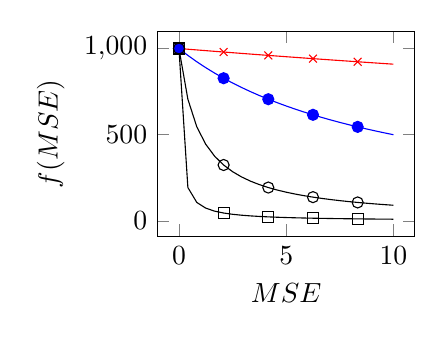
\begin{tikzpicture}[domain=0:10]
    \begin{axis}[xlabel={$MSE$}, ylabel={$f(MSE)$}, width=0.4\linewidth, mark repeat=5, legend entries={{$k=0.01$},{$k=0.1$},{$k=1.0$},{$k=10.0$}}, legend to name=legend_local_refkz, legend columns=4]
      \addplot[mark=x,red]{1000 / (1 + 0.01 * x)};
      \addplot[mark=*,blue]{1000 / (1 + 0.1 * x)};
      \addplot[mark=o,black]{1000 / (1 + 1.0 * x)};
      \addplot[mark=square,black]{1000 / (1 + 10.0 * x)};
    \end{axis}
  \end{tikzpicture}
  \\
  \ref{legend_local_refkz}
  \caption{Графики функции фитнеса для различных значений $k$}
  \label{img:kz}
\end{figure}

\input{cmp_mse_k}

\input{cmp_mse_k_prefix}

\input{cmp_mse_k_overlapped}

В результате экспериментов по символьной регрессии различных наборов данных было выявлено оптимальное значение коэффициента давления отбора~$k=10.0$. Как видно, данная величина отличается от значения, принятого в исходном алгоритме ПЭГ, следовательно, применение данной модификации можно считать успешным. 

%--------------------------------------------------------------------

\subsection{Модификации генетических операторов}

Наибольшим недостатком алгоритма ПЭГ является его склонность к преждевременной сходимости к локальному оптимуму, потому любые техники, направленные на решение этой проблемы, приводят к существенному росту производительности ПЭГ, что выражается в сокращении времени сходимости, улучшении средней приспособленности решений, повышению вероятности успешного обнаружения оптимального решения.

Для усиления способности алгоритма к поиску предлагается~\cite{2008acat.confE.66T} следующий алгоритм динамической мутации DM-GEP. При максимальном количестве поколений $T$ процесс эволюции разбивается на три фазы:
\begin{enumerate}
  \item Начальная фаза: поколения от первого до $T_1$, $0 < T_1 < T$. Вероятность мутации $p_m$ возрастает каждые два поколения со значения 0.022 до 0.44 с шагом 0.001.
  \item Метафаза: поколения от $T_1$ до $T_2$, $T_1 < T_2 < T$. Вероятность мутации $p_m$ возрастает каждые пять поколений со значения 0.022 до 0.66 с шагом 0.002.
  \item Анафаза: поколения от $T_2$ До $T$. Вероятность мутации $p_m$ уменьшается каждые десять поколений со значения 0.066 до 0.022 с шагом 0.001.
\end{enumerate}

В работе~\cite{conf/dews/Tang06} предлагается использовать динамическую установку вероятности мутации, как самого разрушительного оператора, делая ей индивидуальной для каждой особи и зависимой от фитнеса особи. Чем выше фитнес особи, тем более она приспособлена, тем больше внимания требуется уделять локальному поиску, тем меньшая устанавливается вероятность мутации:

\begin{equation}
\label{eq:dynaminc_mutation_probability}
p_m(I) = (1 - f(I) / 1000)*(p_{m_{max}} - p_{m_{min}})+p_{m_{min}}
\end{equation}
где 1000~--- максимальное значение фитнеса, $p_{m_{min}}=0.044$ и $p_{m_{max}}=0.1$~--- нижний и верхний пределы вероятности мутации.

Производительность ПЭГ сильно зависит от заданных вероятностей применения генетических операторов. Снизить влияние этих значений на работу алгоритма возможно путём задействования подхода выбора нового значения, принятого в методе симуляции отжига~\cite{Siwei:2005:pICWCNMC}. Суть применения симуляции отжига состоит во введении зависящего от времени (номера итерации алгоритма) параметра $T$, называемого температурой. Чем выше температура в данный момент времени, тем более вероятна замена исходной особи новой, полученной путём применения генетического оператора. Температура системы уменьшается с каждой последующей итерацией, способствуя поиску окрестностей глобального оптимума на первой фазе алгоритма, и приводя затем к уточнению его местоположения. Скорость понижения температуры управляется аргументом $a$.

На каждой итерации алгоритма ПЭГ к каждой родительской особи $old$ последовательно применяются генетические операторы, каждый из которых порождает новую дочернюю особь $new$. Дочерняя особь занимает место родительской в популяции при выполнении следующего условия:

\begin{equation}
\label{eq:anneal_simulation}
\min(1, e^{-\left\lbrack\frac{f(old) - f(new)}{T_i}\right\rbrack}) > random[0, 1],
\end{equation}
где $f(old)$, $f(new)$~--- фитнесы родительской и дочерней особей соответственно, \mbox{random[0, 1]}~--- случайная величина в диапазоне [0, 1], $T_i$~--- температура на i-той итерации алгоритма. Данная модификация позволила несколько улучшить эффективность ПЭГ.

%--------------------------------------------------------------------

\subsection{Модификации эволюционного процесса}

\subsubsection{Возврат в исходное состояние}

Когда эволюционный процесс проходит определённое количество поколений, средний фитнес популяции достаточно высок, однако разнообразие практически устранено, что приводит к преждевременному схождению к локальному оптимуму, уменьшая шансы успешной глобальной оптимизации. Для решения этой проблемы было предложено~\cite{zhong2006improve} реализовать явление атавизма~--- появление свойств далёких предков. 

Современная генетика описывает следующие причины возникновения атавизмов: рекомбинация утраченного гена предка в результате скрещивания или мутации, и устранение стопового элемента генома, заблокировавшего на определённом этапе экспрессию гена предка. Из природы рассмотренных причин следует обратимость процесса схождения популяции. Кратковременно развернуть процесса эволюции в обратном направлении можно при помощи реализации возврата популяции ПЭГ в исходное состояние (Backtraced GEP).

В основе алгоритма возврата лежит структура данных стек, хранящая <<контрольные точки>>~--- состояния популяции. Если фитнес лучшей особи в новой популяции (полученной в результате репликации и применения генетических операторов), выше, чем у лучшей особи в популяции на верхушке стека (в последней контрольной точке), это означает верное направление эволюции, потому новая популяция заталкивается в стек, формируя новую контрольную точку. В противном случае можно сделать вывод о тупиковой ветви эволюции, потому последняя контролная точка выталкивается из верхушки стека.

Применение методики возврата к предыдущему состоянию привела к значительному улучшению качества получаемых решений.

%--------------------------------------------------------------------

\subsubsection{Обеспечение разнообразния начальной популяции}

Для наиболее эффективного исследования пространства поиска особи начальной популяции должны быть как можно меньше похожи между собой. Создание начальной популяции случайным образом не предполагает никаких процедур по обеспечению генетического разнообразия.

Сравнение особей между собой наиболее удобно производить по генотипу по причине его линейности и лёгкости считывания. Целесообразно при этом сравнивать только кодирующие участки, участвующие в построении синтаксического дерева.

Для количественного измерения близости хромосом между собой в качестве метрики предлагается~\cite{Duan:2007:SID:1304604.1305918} использовать правило, возвращающее максимальное количество $r$ подряд идущих совпадающих элементов. Если две сравниваемые последовательности равны друг другу, $r$ будет равно длине последовательности. Два гена считаются близкими, если значение $r$ превышает определённый порог, авторами использовалось значение 7.
Процедура создания начальной хромосомы с использованием описанной техники выглядит следующим образом:

\begin{enumerate}
  \item Создание пустой популяции.
  \item Создание новой особи случайным образом.
  \item Сравнение этой особи с каждой особью, добавленной в популяцию.
  \item Если новая особь близка какой-либо особи в популяции, перейти к шагу~2, иначе добавить особь в популяцию.
  \item Если популяция полностью заполнена, завершить процедуру, иначе перейти к шагу~2.
\end{enumerate}

Были проведены эксперименты по моделированию различных наборов данных, предоставляемых Лёвенским университетом. Полученные модели обладают б\'{о}льшей корреляцией с тестовыми данными, чем результаты работы исходного алгоритма ПЭГ.

%--------------------------------------------------------------------

\subsubsection{Группировка особей и их параллельная эволюция}

Начиная с определённого поколения, находясь в поздней фазе эволюции, популяция обладает следующими признаками: сложная структура синтаксических деревьев, замедление скорости эволюции, незначительное разнообразие популяции. Однако было замечено~\cite{Jiang:2008:MPT:1473248.1474007}, что разбиение популяции на группы и их параллельная обработка позволяет избежать преждевременной сходимости.

Разбиение популяции на группы происходит следующим образом. Особи популяции сортируются в порядке возрастания значений фитнеса:

\begin{equation}
\label{eq:niches_G}
G = \{I_i | f(I_{i+1}) \ge f(I_i), 1 \le i \le N\}.
\end{equation}

Группой считается последовательность, в которой разница значений фитнесов соседних особей не превышает заданую величину $d$:

\begin{equation}
\label{eq:niches_G_i}
G_i = \{I_j | f(I_{j+1}) - f(I_j) \le d, 1 \le j \le N, 1 \le i \le Q\}
\end{equation}
где $Q$~--- количество образованных групп. Под плотностью группы понимается отношение её размера (количества особей) к размеру популяции:

\begin{equation}
\label{eq:niches_p_i}
p_i = \frac{|G_i|}{N}
\end{equation}

Тогда сумма плотностей групп одной популяции всегда будет равна единице:

\begin{equation}
\label{eq:niches_p_i_sum_1}
\sum\limits_{i=1}^Q{p_i} = 1
\end{equation}

Энтропия популяции, математическое ожидание и дисперсия фитнеса вычисляются таким образом:

\begin{equation}
\label{eq:niches_E}
E(G) = - \sum\limits_{i=1}^Q{p_i \times \log{p_i}}
\end{equation}

\begin{equation}
\label{eq:niches_M}
M(G) = \sum\limits_{i=1}^Q{\hat{f_i} \times p_i}
\end{equation}

\begin{equation}
\label{eq:niches_D}
D(G) = \frac{1}{N} \times \sum\limits_{i=1}^{N}{{f(I_i) - \hat{f}}^2}
\end{equation}

\begin{equation}
\label{eq:niches_f_i_hat}
\hat{f_i} = \frac{1}{|G_i|} \times \sum\limits_{j=1}^{|G_i|}{f(I_j)}
\end{equation}

\begin{equation}
\label{eq:niches_f_hat}
\hat{f} = \frac{1}{N} \times \sum\limits_{i=1}^{N}{f(I_i)}
\end{equation}

Если энтропия и дисперсия популяции меньше определённых заданых пороговых значений, можно сделать вывод о недостаточной степени генетического разнообразия. В этом случае имеет смысл заменить худшие 10\% особей новыми, созданными случайным образом. Указанные операции требуется применять к каждому поколению. Итоговый алгоритм работы алгоритма представлен в листинге~\ref{algo:niches}.

\begin{algorithm}
\SetAlgoLined
\While{Не достигнуто максимальное поколение}
{
  Создание начальной популяции\;
  Разбиение популяции на группы\;
  \ForEach{группы популяции}
  {
    Перенос лучшей особи\;
    Применение генетических операторов\;
  }
  Расчет энтропии и дисперсии популяции\;
  Замена худших особей популяции при необходимости\;
  Разбиение популяции на группы\;
}
Вывести лучшую особь\;
\caption{Алгоритм ПЭГ с группировкой особей}
\label{algo:niches}
\end{algorithm}

Авторами не было произведено сравнение производительности полученной системы с исходным ПЭГ или другими его модификациями.

Вляние отдельно взятой модификации, удаляющие худшие особи, показано в таблице~\ref{tbl:cmp_replace_worst}. Из этих результатов следует изменение баланса двух основных вероятностных показателей алгоритмов: улучшается точность наилучшей возможной модели при большом количестве запусков, но в то же время страдает вероятность обнаружения приемлемого решения.

\input{cmp_replace_worst}

%--------------------------------------------------------------------

\subsubsection{Комбинация моделей}

Полученные в ходе нескольких запусков алгоритма ПЭГ модели можно~\cite{journals/jikm/AbrahamG06, guo2012novel} обобщить в одну, представляя итоговую формулу в виде:
\begin{equation}
\label{eq:ensembles}
M = a \times M_1 + b \times M_2 + c \times M_3 + \ldots
\end{equation}
где $a$, $b$, $c$, $\ldots$~--- комбинирующие коэффициенты, $M_1$, $M_2$, $M_3$, $\ldots$~--- модели, полученные в ходе запусков ПЭГ.

Для подобра комбинирующих коэффициентов с целью минимизации погрешности итоговой модели, повышению её корреляции с выборками данных был использован генетический алгоритм NSGA II (non-dominated sorting genetic algorithm II).

Как правило, обобщающая модель обладает лучшими характеристиками, чем её составляющие по отдельности.

%--------------------------------------------------------------------

\subsection{Популяции неоднородных особей}

Одна из проблем алгоритма ПЭГ~--- определение оптимального размера головы гена (и размера решения). Из-за отсутствия процедуры априорного задания приходится запускать алгоритм множество раз с разными параметрами для поиска наиболее подходящих. В качестве другого способа предлагается~\cite{Lopes:2004:AMCS} использовать в одной популяции хромосомы различной длины: половина популяции заполняется особями пропорционально с диапазоном размеров, заданным пользователем, длина генов особей второй половины устанавливается случайным образом. Операторы рекомбинации в таком случае применяются только к особям с хромосомами равной длины.

Для подстройки констант предлагается использовать градиентный алгоритм, обладающий высокой вычислительной стоимостью, потому применяющийся с определённой вероятностью. Константа либо заменяется случайно выбранной, либо изменяется в пределах 10\%. Если мутированная особь лучше исходной, то заменяет её, иначе константа заменяется полусуммой последних двух значений. Процесс повторяется до тех пор, пока мутировавшая особь не будет хуже исходной, либо по достижении предела в 10 итераций.

Аналогичные исследования проведены в работе~\cite{journals/acisc/BrowneS10}. Предложено использовать хромосомы с переменным числом генов и переменным размером каждого гена. Введены новые операторы, направленные на изменение длины генома:
\begin{itemize}
  \item Удаление одного ген из хромосомы.
  \item Создание и добавление одного нового гена в хромосому.
  \item Перенос участка головы одного гена в голову другого, что приводит к укорачиванию первого и удлиннению второго.
  \item Рекомбинация разнородных хромосом.
\end{itemize}

Такой подход привёл к двукратному сокращению длины гена и, соответственно, размера синтаксического дерева решения.
